\section{Servoberäkningar}

Servoberäkningarna tillkommer som underlag för objektidentifieringsdelen. Nedan behandlas samtliga beräkningar för de fyra servon som styr tummen och pekfingret. 

\subsection{Beräkningar för servo 1}

Servo 1 är med hjälp av ett stag kopplat till tummens första led och styr därmed dess $\alpha$ vinkel (se \ref{fig:servo1})

\begin{figure}[H]
\label{fig:servo1}
\includegraphics[width=0.7\textwidth]{img/servo/servo_berakning11}
\caption{Rörelse i tummens första led till följd av rörelse i servo 1}
\end{figure}

Bild \ref{fig:servo2} nedan visar hur servot är kopplat via ett stag till tummens första led. Servot har sin roterande axel i punkt $P_{0}$ vilken sedan är förskjutet till punkt $P_{1}$ med hjälp av ett servokors med radie $R_{1}$. Servokorset drar i sin tur i ett stag med längden c som påverkar tummens första led. Leden kan rotera kring punkt $P_{3}$ vilket ger upphov till en vinkel $\alpha$.


\begin{figure}[H]
\label{fig:servo2}
\includegraphics[width=0.6\textwidth]{img/servo/servo1}
\caption{Nödvändiga beteckningar för beräkningar till servo 1}
\end{figure}

\[
\begin{cases}
r_{1}=\unit[16]{mm} \\
r_{2}=\unit[12]{mm}\\
a=\unit[4]{mm}\\
b=\unit[55]{mm}\\
c=\unit[58]{mm} \\
\end{cases}
\]

\begin{table}[H]
    \begin{tabular}{|c|l|l|}
        \hline
        Punkt  & X-Koordinat                          & Y-Koordinat                          \\ \hline
        $P_{0}$      & 0                                    & 0                                   \\ \hline
        $P_{1}$      & $r_{1}\cos(\phi)$              & $r_{1}\sin(\phi)$              \\ \hline
        $P_{2}$      & $P_{3x}-r_{2}\sin(\alpha)$                  & $P_{3y}+r_{2}\cos(\alpha)$                  \\ \hline
        $P_{3}$      & $b$ & $-a$ \\
        \hline
    \end{tabular}
\end{table}



Avståndet mellan punkterna $P_{2}$ och $P_{1}$ är  alltid c vilket är längden på staget som sammankopplar de båda punkterna. Detta utnyttjas för att upprätta ett itterations villkor. Ett gissat värde på alfa ($\alpha_{guess}$) ger koordinaterna för punkt $P_{2}$ vilket ger ett avstånd mha avståndsformeln (se itterationsschemat nedan). På så sät kan ett specifikt $\alpha$ fås för varje servo vinkel $\phi$



\begin{flushleft}

 (1)   $\phi,\alpha_{guess}$ $\rightarrow$ \\ 
  (2)  $P_{1}=[r_{1}\cos(\phi),r_{1}\sin(\phi)]$ $\rightarrow$
  \\(3) \thinspace $P_{2}=[P_{3x}-r_{2}\sin(\alpha_{guess}),P_{3y}+r_{2}\cos(\alpha_{guess})]$ $\rightarrow$ \\
  (4)\ $c_{g}=\sqrt[]{(P_{1x}-P_{2x})^2+(P_{1y}-P_{2y})^2}$ $\rightarrow$\\(5) Kolla om: $|c-c_{g}|>tol$ \\ (6) Om (5) stämmer $\rightarrow$ $\alpha_{guess}=\alpha_{guess}+value$ \ , \ börja om från punkt (3) \\ annars $\rightarrow$ det approximativa $\alpha$-värdet har hittats
\end{flushleft}

Med hjälp av matlab så har ovanstående itterationsshema genererat ett $\alpha$-värde för varje servoläge ($\phi$). Detta utnyttjades sedan med minsta kvadratmetoden för att ta fram ekvation \eqref{eq:servo1} från dessa värden. 

\begin{equation}
\label{eq:servo1}
\alpha= A\phi^4+B\phi^3+C\phi^2+D\phi+E
\end{equation}

\begin{table}[H]
    \begin{tabular}{|c|l|}
        \hline
        A      & 0.000005730076566  \\ \hline
        B      & -0.000776743538556  \\ \hline
        C      & 0.050190358704910    \\ \hline
        D      & -0.929487032616965    \\ \hline
        E      & 5.269186999542453      \\ \hline
    \end{tabular}
\end{table}


\begin{figure}[H]
\label{servo3}
\includegraphics[width=0.7\textwidth]{img/servo/servo1_alfa}
\caption{$\alpha$-vinkeln som en funktion av servovinkeln $\phi$}
\end{figure}

Genom att anpassa en ekvation till kurvan undviks itterations processen vid styrning av handen vilket underlättar för processon. Med hjälp av ekvation \eqref{eq:servo2} kan koordinaterna för ytterpunkterna på tummens första led beräknas. Tummens origo är placerat i dess första roterande punkt, punkt $P_{3}$ (se \ref{fig:servo2})

\begin{equation}
\label{eq:servo2}
P1_{tumme}=[L_{1}\sin(\alpha),L_{1}\cos(\alpha)] 
\end{equation}


\begin{center}
$(L_{1}=39mm)$
\end{center}



\subsection{Beräkningar för servo 2}

Servo 2 styr tummens andra led (se \ref{fig:servo4}) genom att applicera en kraft på en sena kopplat till ledens mittpunkt(punkt $P_{2}$ se\ref{fig:servo5}).

\begin{figure}[H]
\label{fig:servo4}
\includegraphics[width=0.7\textwidth]{img/servo/servo_berakning2}
\caption{Rörelse i tummens andra led till följd av rörelse i servo 2}
\end{figure}

\begin{minipage}[t]{0.5\textwidth}
\begin{figure}[H]
\label{fig:servo5}
\includegraphics[width=0.8\textwidth]{img/servo/servo_berakning22}
\caption{}
\end{figure}
\end{minipage}
\begin{minipage}[t]{0.5\textwidth}
\begin{figure}[H]
\label{fig:servo6}
\includegraphics[width=1\textwidth]{img/servo/servo_berakning23}
\caption{}
\end{figure}
\end{minipage}